%%%%%%%%%%%%%%%%%%%%%%%%%%%%%%%%%%%%%%%%%%%%%%%%%%%%%%%%%%%%%%%%%%%%%%
% Problem statement
\begin{statement}[
  problempoints=110,
  timelimit=1 sekunda,
  memorylimit=512 MiB,
]{Skandi}

%\setlength\intextsep{-0.1cm}
%\begin{wrapfigure}[7]{r}{0.27\textwidth}
%\centering
%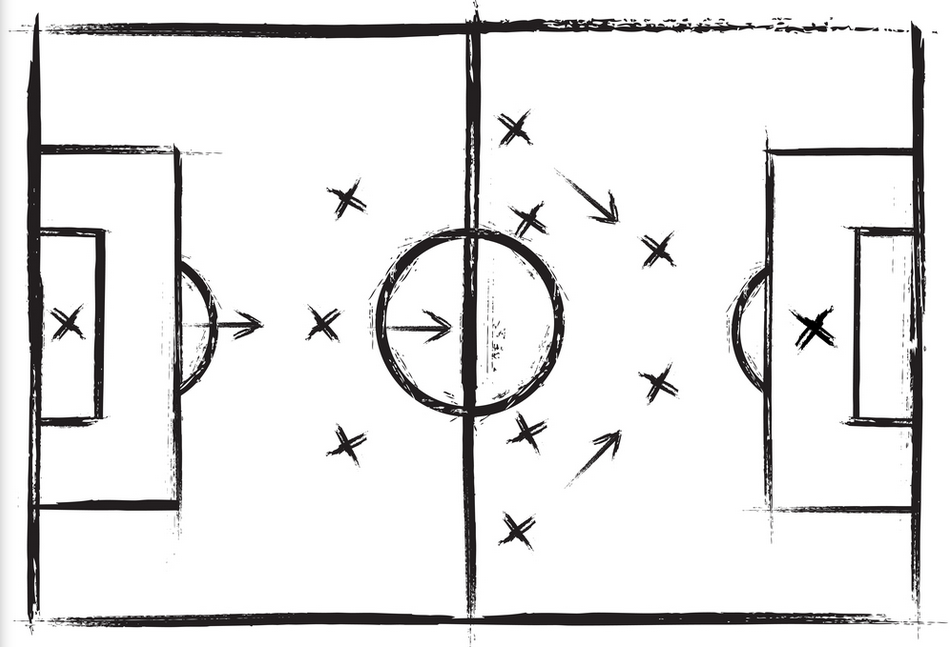
\includegraphics[width=0.27\textwidth]{img/trener.png}
%\end{wrapfigure}

Dragica je predsjednica treće podružnice Udruge umirovljenika grada Samobora,
strastvena kuharica te vjerojatno jedna od najboljih rješavateljica
skandinavki u Hrvatskoj. Skandinavka je pravokutna križaljka dimenzija $N
\times M$ u kojoj su polja ili prazna (te se trebaju popuniti) ili ispunjena.
Ispunjena polja sadrže najviše dva pitanja, jedno na koje se odgovara prema
desno i drugo na koje se odgovara prema dolje. Odgovori na pitanja upisuju se
na prazna polja prema dolje ili prema desno od polja na kojem se nalazi
pitanje do idućeg ispunjenog polja ili do ruba križaljke.  Pitanje prema
desno će uvijek postojati osim ako je blokirano rubom skandinavke ili
ispunjenim poljem zdesna. Analogno, pitanje prema dolje će uvijek postojati
osim ako je blokirano rubom skandinavke ili ispunjenim poljem odozdo

Dragica zna odgovoriti na sva pitanja u skandinavki, ali je svjesna da joj nije
preostalo još puno vremena pa želi odgovoriti \textbf{na što manje pitanja, a
da ispuni cijelu skandinavku}. Nažalost, ona ne zna na koliko pitanja
minimalno mora odgovoriti te koja će to pitanja biti pa zato traži svoje
najdraže unuke da joj pomognu.

%%%%%%%%%%%%%%%%%%%%%%%%%%%%%%%%%%%%%%%%%%%%%%%%%%%%%%%%%%%%%%%%%%%%%%
% Input
\subsection*{Ulazni podaci}
U prvom su retku prirodni brojevi $N$ i $M$ $(2 \le N, M \le 500)$, iz teksta
zadatka.

U sljedećih se $N$ redaka nalazi po $M$ znakova \texttt{‘0’} ili
\texttt{‘1’}, gdje \texttt{‘0’} predstavlja prazno polje koje treba popuniti,
a \texttt{‘1’} predstavlja ispunjeno polje . Kao i u pravim skandinavkama,
vrijedi da će prvi red i stupac biti popunjeni znakovima \texttt{‘1’}.

Garantiramo da će postojati barem jedno polje s oznakom \texttt{‘0’}.

%%%%%%%%%%%%%%%%%%%%%%%%%%%%%%%%%%%%%%%%%%%%%%%%%%%%%%%%%%%%%%%%%%%%%%
% Output
\subsection*{Izlazni podaci}
U prvom retku treba ispisati najmanji mogući broj pitanja na koja se mora
odgovoriti da bi se popunila cijela skandinavka. Označimo taj broj s $X$.

U sljedećih $X$ redaka treba ispisati na koja pitanja Dragica mora odgovoriti.
Ispis je oblika: \texttt{R S smjer}, gdje je $R$ oznaka reda u kojem se
nalazi pitanje, $S$ oznaka stupca i smjer jedna od riječi \texttt{"DESNO"}
ili \texttt{"DOLJE"}.

Ako postoji više mogućih rješenja, ispišite bilo koje.

%%%%%%%%%%%%%%%%%%%%%%%%%%%%%%%%%%%%%%%%%%%%%%%%%%%%%%%%%%%%%%%%%%%%%%
% Scoring
\subsection*{Bodovanje}
{\renewcommand{\arraystretch}{1.4}
  \setlength{\tabcolsep}{6pt}
  \begin{tabular}{ccl}
 Podzadatak & Broj bodova & Ograničenja \\ \midrule
  1 & 18 & Bit će najviše $9$ polja s oznakom \texttt{'1'} \\
  2 & 32 & $N \le 500$ i $M \le 10$\\
  3 & 60 & Nema dodatnih ograničenja. \\
\end{tabular}}

Ako vaše rješenje ispiše točan prvi redak na svim testnim primjerima nekog
podzadatka, ali na barem jednom testnom primjeru neispravno ispiše preostale
retke, osvojit ćete $50$\% bodova predviđenih za taj podzadatak.

%%%%%%%%%%%%%%%%%%%%%%%%%%%%%%%%%%%%%%%%%%%%%%%%%%%%%%%%%%%%%%%%%%%%%%
% Examples
\subsection*{Probni primjeri}
\begin{tabularx}{\textwidth}{X'X'X}
\sampleinputs{test/skandi.dummy.in.1}{test/skandi.dummy.out.1} &
\sampleinputs{test/skandi.dummy.in.2}{test/skandi.dummy.out.2} &
\sampleinputs{test/skandi.dummy.in.3}{test/skandi.dummy.out.3}
\end{tabularx}

\textbf{Pojašnjenje trećeg probnog primjera:}
Primjer prave skandinavke koja je ekvivalentna ovom probnom primjeru prikazan
je na idućoj stranici. Ispunjena polja označena su crnom bojom, a polja koja
sadrže barem jedno pitanje su dodatno numerirana. Ispod slike prikazana su
pitanja koja se rješavaju prema desno (stupac "vodoravno") i pitanja koja se
rješavaju prema dolje (stupac "okomito"). Primijetite da neka ispunjena polja
sadrže samo jedno pitanje (primjerice polja $8$ i $13$), dok neka ispunjena
polja sadrže po dva pitanja (primjerica poja $10$ i $12$). Ovu konkretnu
skandinavku moguće je u potpunosti riješiti ako znamo odgovore na $14$ pitanja
koja su navedena u izlazu probnog primjera. Okušajte se sami!

\setlength\intextsep{-0.5cm}
\begin{wrapfigure}{c}{\textwidth}
\centering
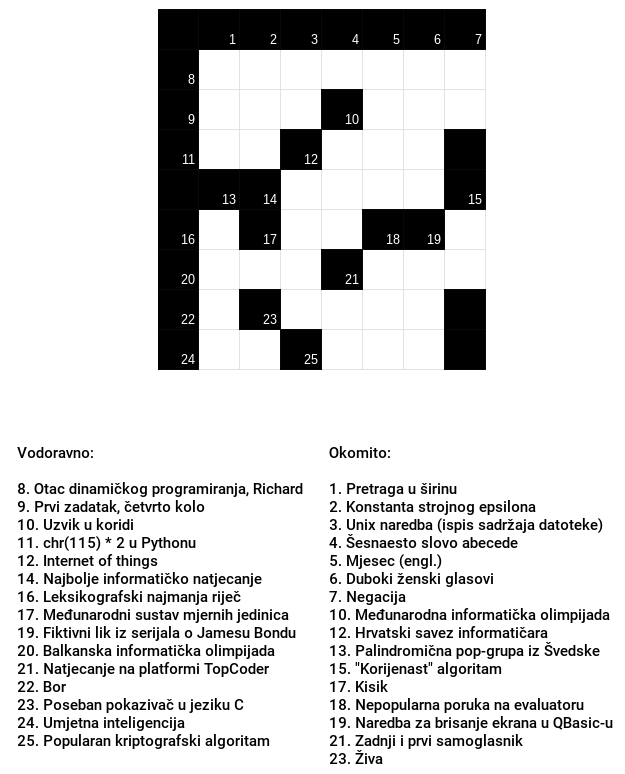
\includegraphics[width=0.8\textwidth]{skandi.png}
\end{wrapfigure}

%%%%%%%%%%%%%%%%%%%%%%%%%%%%%%%%%%%%%%%%%%%%%%%%%%%%%%%%%%%%%%%%%%%%%%
% We're done
\end{statement}

%%% Local Variables:
%%% mode: latex
%%% mode: flyspell
%%% ispell-local-dictionary: "croatian"
%%% TeX-master: "../hio.tex"
%%% End:
